\documentclass[11pt,a4paper]{article}
\usepackage[margin=1in]{geometry}
\usepackage[T1]{fontenc}
\usepackage{enumitem}
\usepackage{titlesec}
\usepackage{parskip}
\usepackage{setspace}
\usepackage{array}
\usepackage{xcolor}
\usepackage{graphicx}
\usepackage{tikz}
\usetikzlibrary{arrows.meta, positioning, fit, backgrounds}

\setstretch{1.1}
\pagestyle{empty}
\setlist{itemsep=0.25em,topsep=0.3em,leftmargin=1.5em}
\titleformat{\section}{\large\bfseries\color{green!40!black}}{\thesection.}{0.5em}{}
\titlespacing*{\section}{0pt}{1.4em}{0.5em}

\begin{document}


\vspace{0.6em}

\begin{center}
{\LARGE\bfseries\textcolor{green!40!black}{Green Customer Insights Platform}}
\end{center}

\vspace{1.3em}
{\color{green!45!black}\hrule height 1.2pt}
\vspace{0.5em}

\section{Problem Statement and Understanding}
The challenge is to build an AI-powered platform for Lloyds that turns customer transactions, product holdings and behavioural data into actionable green financial opportunities. Four product recommendations are required (EV Finance, Green Home Loan, Solar Finance, Paperless Banking) and two are optional (Green Investments, Green Loans).

We see three constraints that shape the whole design:
\begin{itemize}
  \item \textbf{Separation of concerns.} ML models only predict propensity. A deterministic carbon engine computes environmental impact from documented formulas. Eligibility comes from bank product rules. The LLM is limited to turning structured outputs into plain language.
  \item \textbf{Guardrails and eligibility.} A propensity score or behavioural signal never establishes eligibility. Negative guardrails block illogical or redundant offers, e.g.\ no EV finance for a customer who already owns an EV or has a car loan.
  \item \textbf{Explainability.} Each recommendation must carry supporting evidence, a confidence rating, fixed reason codes and data timestamps.
\end{itemize}

\section{Idea and Abstract}
We propose a modular, end-to-end pipeline, the Green Customer Insights Platform. It ingests transaction logs, demographics and financial holdings and builds a unified Customer 360 view per customer.

Transactions are categorised into mutually exclusive sustainability buckets: Fuel, Electricity, Gas, Public Transport, Home Improvement, Automotive, Utilities and Other. A supervised classifier predicts product propensities, and a deterministic carbon engine estimates projected annual CO$_2$e reduction using standard emission factors. A structured LLM layer then writes personalised customer-facing explanations, while a dashboard shows portfolio trends, high-potential segments and conversion metrics for relationship managers.

\section{Product Signals and Guardrails}
Each required product is driven by specific behavioural signals and blocked by specific holdings. These are our planned rules; thresholds will be tuned on the data.

\begin{center}
\small
\begin{tabular}{|p{3.2cm}|p{5.5cm}|p{5.9cm}|}
\hline
\textbf{Product} & \textbf{Signals (propensity input)} & \textbf{Negative guardrail} \\ \hline
EV Finance & Fuel and Automotive spend, public transport use, income band & Already owns an EV or has a car loan \\ \hline
Green Home Loan & Home Improvement spend, utility bills, existing mortgage profile & Existing green home loan; fails eligibility rules \\ \hline
Solar Finance & High Electricity spend, home ownership signals & Already holds solar finance; no home ownership \\ \hline
Paperless Banking & Digital transaction share, app activity & Already paperless \\ \hline
\end{tabular}
\end{center}

\newpage

\section{High-Level Approach and Architecture}
The system runs through five sequential stages:

\begin{figure}[htbp]
\centering
\resizebox{\textwidth}{!}{%
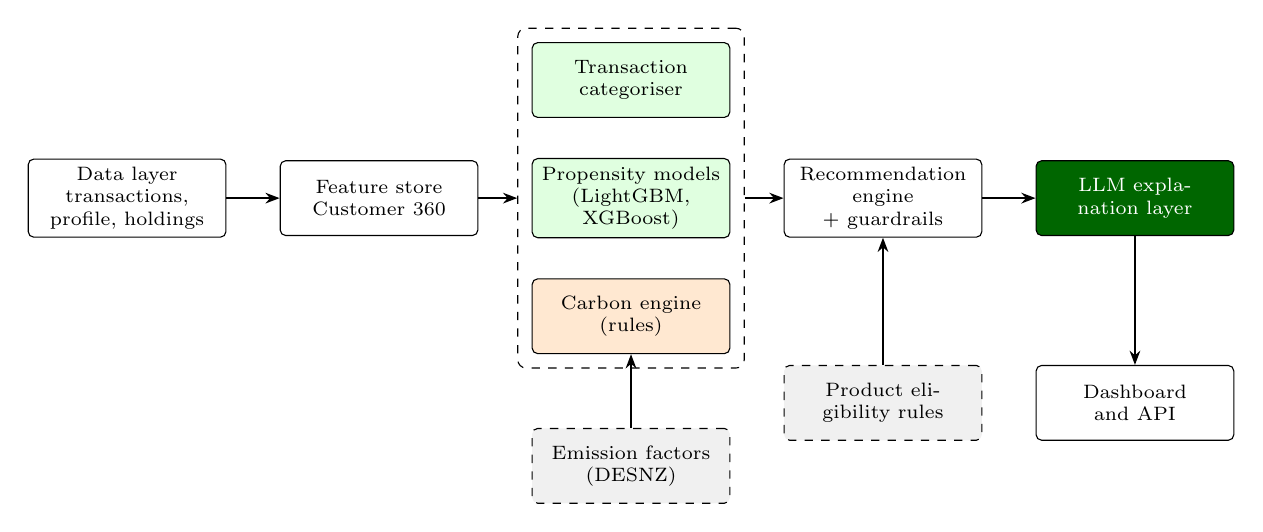
\begin{tikzpicture}[
  box/.style={
    draw, rounded corners=2pt, align=center,
    font=\scriptsize, text width=2.3cm,
    minimum height=0.95cm, inner sep=3pt, fill=white
  },
  ext/.style={box, dashed, fill=gray!12},
  llm/.style={box, fill=green!40!black, text=white},
  arr/.style={-{Stealth[length=1.8mm]}, thick}
]
\node[box] (data) at (0,0)
  {Data layer\\transactions, profile, holdings};
\node[box] (fs) at (3.2,0)
  {Feature store\\Customer 360};
\node[box, fill=green!12] (cat) at (6.4,1.5)
  {Transaction categoriser};
\node[box, fill=green!12] (ml) at (6.4,0)
  {Propensity models\\(LightGBM, XGBoost)};
\node[box, fill=orange!18] (co2) at (6.4,-1.5)
  {Carbon engine\\(rules)};
\node[box] (rec) at (9.6,0)
  {Recommendation engine\\+ guardrails};
\node[llm] (llm) at (12.8,0)
  {LLM explanation layer};
\node[box] (dash) at (12.8,-2.6)
  {Dashboard and API};
\node[ext] (ef) at (6.4,-3.4)
  {Emission factors\\(DESNZ)};
\node[ext] (rules) at (9.6,-2.6)
  {Product eligibility rules};

\begin{scope}[on background layer]
  \node[
    draw, dashed, rounded corners=3pt,
    fit=(cat)(ml)(co2), inner sep=5pt
  ] (grp) {};
\end{scope}

\draw[arr] (data) -- (fs);
\draw[arr] (fs) -- (grp);
\draw[arr] (grp) -- (rec);
\draw[arr] (rec) -- (llm);
\draw[arr] (llm) -- (dash);
\draw[arr] (ef) -- (co2);
\draw[arr] (rules) -- (rec);
\end{tikzpicture}%
}
\vspace{0.4em}

{\small\textcolor{green!40!black}{
Figure 1. Green Customer Insights Platform architecture.
Dashed boxes denote reference inputs and parallel processing components.
}}
\end{figure}

\begin{enumerate}
  \item \textbf{Data ingestion and feature store.} Join transaction data with customer profile and loan holding attributes. Create clean customer-level train, validation and test splits so no customer appears in more than one split (prevents leakage).
  \item \textbf{Categorisation and Customer 360.} Merge the tables into one view per customer. Map merchant descriptions to the sustainability categories using deterministic keyword rules and regex.
  \item \textbf{Propensity and carbon engines.}
  \begin{itemize}
    \item \emph{ML models:} LightGBM and XGBoost classifiers output a propensity probability, a confidence metric and fixed reason codes for each required green product.
    \item \emph{Carbon engine:} rules-based; computes avoided emissions (e.g.\ current transport emissions versus post-EV adoption) using documented GHG Protocol factors.
  \end{itemize}
  \item \textbf{Recommendation and guardrails.} Apply negative guardrails on existing holdings and eligibility rules to remove ineligible or redundant recommendations.
  \item \textbf{Presentation layer.} Pass structured JSON to an LLM for customer-facing explanations, and render an interactive Streamlit dashboard for portfolio-level analytics.
\end{enumerate}

\section{Planned Testing Methodology}
\begin{itemize}
  \item \textbf{Baseline comparison.} Benchmark the ML models against a simple rule-based heuristic (e.g.\ targeting customers by a high single-category spend threshold) to show predictive lift.
  \item \textbf{Held-out metrics.} Evaluate on customer-level validation splits using ROC-AUC, PR-AUC and F1, since classes are imbalanced.
  \item \textbf{Scenario and stress tests.} Test missing or sparse transaction logs, conflicting customer data, and guardrail triggers (customers with existing green holdings must be blocked from redundant offers).
  \item \textbf{Reproducibility.} Preprocessing, training and inference scripts will be runnable from the repository with fixed seeds, and containerised.
\end{itemize}

\section{Explainable Output and Dashboard}
For every customer-product pair the system emits one structured record: product, propensity score, confidence rating, reason codes, supporting evidence (the spend categories and values used), projected CO$_2$e saving, eligibility status and a data timestamp. The LLM only rewrites this record as plain language and may not add facts or change numbers. The dashboard aggregates the same records into portfolio emissions by category, high-potential segments, and expected conversion per product for relationship managers.

\end{document}
